\documentclass[10pt]{article}
\usepackage[a4paper,margin=1.9cm]{geometry}
\usepackage{amsmath,amssymb}
\usepackage{graphicx}
\graphicspath{{../}{./}}
\usepackage{float}
\usepackage[dvipsnames]{xcolor}
\usepackage{enumitem}
\usepackage{titlesec}
\usepackage[hidelinks]{hyperref}

% --- compact layout ---
\setlist[itemize]{leftmargin=1.35em,itemsep=1pt,topsep=2pt,parsep=0pt}
\setlength{\parindent}{0pt}
\setlength{\parskip}{3pt}
\titlespacing*{\section}{0pt}{6pt}{3pt}
\titlespacing*{\subsection}{0pt}{4pt}{2pt}
\titleformat{\section}{\normalfont\large\bfseries\color{RoyalBlue}}{\thesection.}{0.5em}{}
\titleformat{\subsection}{\normalfont\bfseries}{}{0em}{}

\newcommand{\code}[1]{\texttt{\small #1}}
\newcommand{\file}[1]{\textcolor{RoyalBlue}{\texttt{\small #1}}}

% \docheader{title}{subtitle}
\newcommand{\docheader}[2]{%
  \begin{center}
    {\LARGE\bfseries #1}\\[2pt]
    {\small #2}
  \end{center}
  \vspace{-4pt}\hrule\vspace{6pt}
}

\begin{document}

\docheader{Adora --- MLP Equation of State}%
{As-built notes \quad$\cdot$\quad Ivan Milic \quad$\cdot$\quad 2026-09-19 \quad$\cdot$\quad session summary}

Built \file{eos\_mlp/}: a tiny differentiable MLP surrogate for the \textbf{LTE equation of state}, so
the electron density \code{ne} and total hydrogen density \code{nHtot} are no longer passed as free,
degenerate RT inputs but recovered from the real thermodynamic state. Trained once on a Wittmann grid;
inference is pure JAX and portable (no \code{lightweaver} at use time).

\subsection*{1. Concept}
The MLP learns a single scalar, the electron pressure \code{Pe}, versus two thermodynamic variables. The
primary head is $(T, P_\mathrm{gas})\!\to\!P_e$ (used for \emph{both} synthesis and inversion); a second
$(T,\rho)\!\to\!P_e$ head is kept as an optional convenience. Everything the RT needs then follows
algebraically:
\[
n_e = \frac{P_e}{k_B T},\qquad
n_{\mathrm H,\mathrm{tot}} = \frac{P_\mathrm{gas}-P_e}{k_B T\,\Sigma_A},\qquad
\Sigma_A=\textstyle\sum_i n_i/n_\mathrm H = 1.095 .
\]
This replaces the two loosely-constrained free parameters $(n_e, n_{\mathrm H,\mathrm{tot}})$ with one
physical variable, $P_\mathrm{gas}$, per depth.

\subsection*{2. Ground truth \& grid}
Ground truth is \code{lightweaver.wittmann.Wittmann} --- a full multi-element LTE Saha--Boltzmann EOS
(Kurucz partition functions, metal electron donors, molecules; CGS, scalar). Tabulated on a
$96\times96$ grid over $T\in[3\times10^3,5\times10^4]$\,K and $P_\mathrm{gas}\in[10^{-3},10^{7}]$
dyn/cm$^2$ (photosphere + chromosphere regime), 0 bad corners, $\sim$25\,s. \code{lightweaver} is a
\textbf{data-generation-time dependency only}; the trained model is pure JAX.

\subsection*{3. Model \& training}
Deliberately small: random Fourier features ($N{=}32$) $\to$ MLP $64\times64$, \code{tanh}, fp64. Fits
$\log_{10}P_e$ in normalized CGS log space (SI is converted at the API boundary). Trained with
\code{optax} Adam, 20k steps/head, $\sim$4\,min on CPU.

\subsection*{4. Accuracy --- validated}
Relative error in $P_e$ (equivalently $n_e$, since $n_e\propto P_e$): \textbf{median 0.44\%}
($P_\mathrm{gas}$ head) / 0.35\% ($\rho$ head), max $\sim$3--4\% at the sharp hydrogen-ionization ridge;
the error map is spatially uniform (fit noise, no systematic miss). Against FAL-C the model reproduces
$n_e$ to \textbf{$<$0.1\%} in the photosphere where LTE holds, and diverges only in the upper
chromosphere where FAL-C's $n_e$ is NLTE hydrogen-ionization-enhanced --- as an LTE EOS must. Gradients
are finite (\code{jax.grad} verified); the API is \code{jit}/\code{vmap}/\code{grad}-safe.

\begin{center}
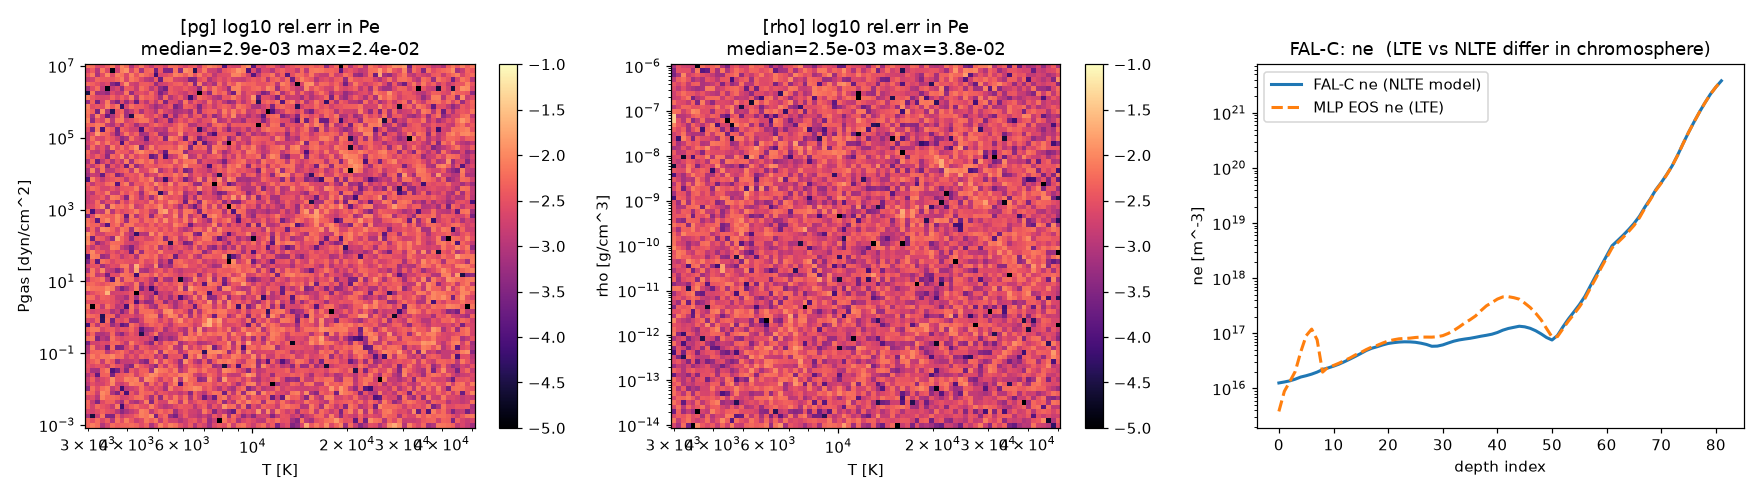
\includegraphics[width=0.95\linewidth]{eos_validation.png}\\[2pt]
{\small\itshape Left/middle: $\log_{10}$ relative error in $P_e$ vs Wittmann across the grid
(\code{pg}, \code{rho} heads). Right: FAL-C $n_e$ --- MLP (LTE) tracks the model in the photosphere and
deep layers, differs in the NLTE chromosphere as expected.}
\end{center}

\subsection*{5. Files (all in \file{eos\_mlp/})}
\file{eos\_config.py} (ranges/units), \file{generate\_grid.py} (Wittmann $\to$ grids; needs
lightweaver), \file{eos\_model.py} (pure-JAX MLP), \file{train\_eos.py} (one-time training),
\textbf{\file{eos.py}} (portable inference, SI in/out), \file{validate\_eos.py}, \file{README.md}.
Artefacts: \file{eos\_grid\_\{pg,rho\}.npz}, \file{eos\_\{pg,rho\}.npz}, \file{eos\_validation.png}.

\subsection*{6. Use \& next}
\code{ne, nHtot = eos.ne\_nhtot\_from\_pg(eos.load\_eos("pg"), T, Pgas)}, then feed
\code{lte\_polarised\_rt(...)} --- the RT needs \textbf{no change} (it already takes \code{ne},
\code{nhtot} in SI). \textbf{Next:} wire the \code{pg} head into the inversion (one \code{Pgas} node per
depth in place of free \code{ne}/\code{nhtot}) and into \file{synth3d.py}. Files are currently
uncommitted.

\end{document}
